\section{Learned Feature Importances}
\label{sec:param_importance}

\subsection{ScoNe}
\begin{figure}[H]
  \centering
  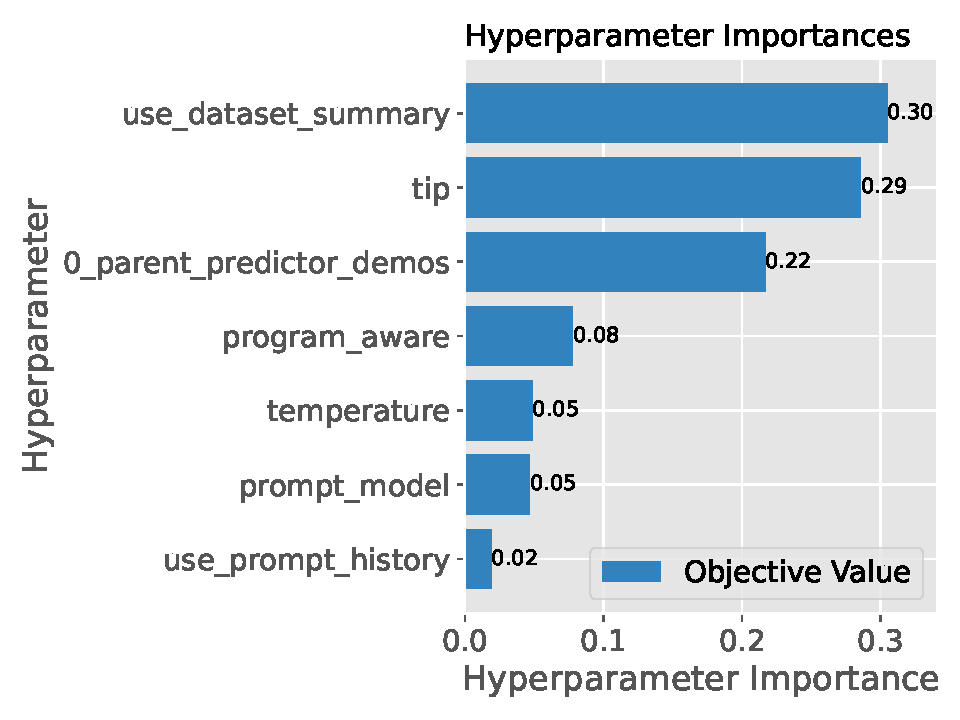
\includegraphics[width=0.4\textwidth]{figures/ScoNe_importance_plots.pdf}
  \caption{Learned hyperparameter importances for ScoNe. Here we see that the Bayesian model learned the dataset summary, the tip, and the task demos in the prompt to be important to proposal quality.}
  \label{fig:scone_importance}
\end{figure}

\subsection{HotpotQA}
\begin{figure}[H]
  \centering
  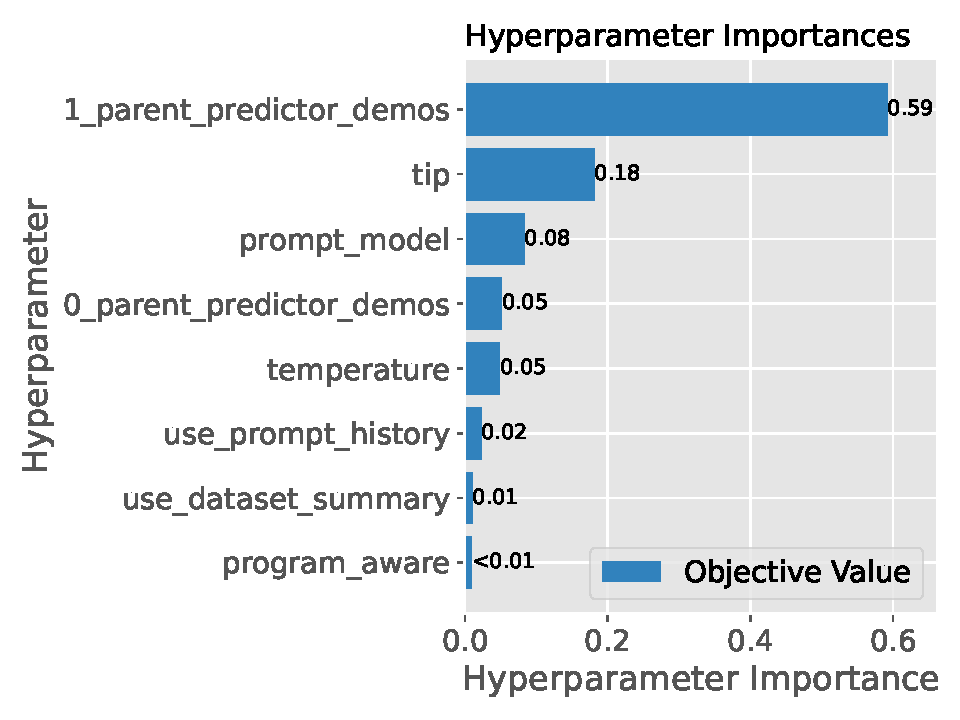
\includegraphics[width=0.4\textwidth]{figures/HotpotQA_importance_plots.pdf}
  \caption{Learned hyperparameter importances for HotpotQA. Here we see that the set of demonstrations chosen for the meta-prompt were most important for proposal quality.}
  \label{fig:hotpot_hyperparams}
\end{figure}

\subsection{HoVeR}
\begin{figure}[H]
  \centering
  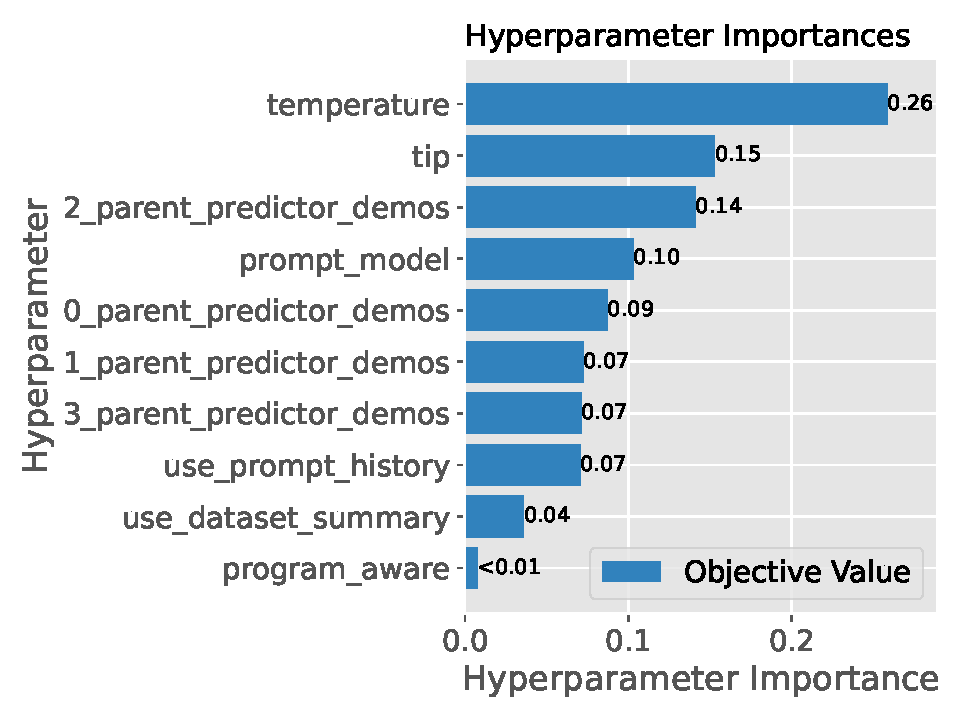
\includegraphics[width=0.4\textwidth]{figures/HoVeR_importance_plots.pdf}
  \caption{Learned hyperparameter importances for HoVeR. Again, we see that the task demonstrations chosen (ie. the parent predictor demos, as labeled here for each module in the program) are learned to be important, as well as the tip. In this case, we also see that the proposal temperature is learned to be important to the model.}
  \label{fig:hover_hyperparams}
\end{figure}

